% answers.tex —— 2015 年·全国Ⅰ卷·文科 · 参考答案与详细解析片段
% 由 tools/generate_projects.py 依来源总账自 2015/2015_数学真题_全国1文_试题.md + 2015/2015_数学真题_全国1文_解析正文.md + 2015/2015_数学真题_全国1文_答案要点.md 生成，勿手改（改源 MD 后重跑）


\begin{gktip}
项目独立推导与盲核，非官方解析。除第 23 题 (2) 为 U 外，其余为 D；源表 \texttt{1.469} 保留。
\end{gktip}

\begin{answer}
\gksolhead{1}{}

\textbf{题目}：

已知集合 $A=\{x\mid x=3n+2,n\in\mathbf N\}$，$B=\{6,8,10,12,14\}$，则集合 $A\cap B$ 中的元素个数为（　）

(A) 5　(B) 4　(C) 3　(D) 2

\Needspace{4\baselineskip}
\textbf{解析}

在 $B$ 中满足 $x\equiv2\pmod3$ 的数为 8、14，故交集有 2 个元素。

\gkanswer{答案：D，$2$}

\end{answer}
\begin{answer}
\gksolhead{2}{}

\textbf{题目}：

已知点 $A(0,1)$，$B(3,2)$，向量 $\overrightarrow{AC}=(-4,-3)$，则向量 $\overrightarrow{BC}=$（　）

(A) $(-7,-4)$　(B) $(7,4)$　(C) $(-1,4)$　(D) $(1,4)$

\Needspace{4\baselineskip}
\textbf{解析}

$C=A+\overrightarrow{AC}=(-4,-2)$，故 $\overrightarrow{BC}=C-B=(-7,-4)$。

\gkanswer{答案：A，$(-7,-4)$}

\end{answer}
\begin{answer}
\gksolhead{3}{}

\textbf{题目}：

已知复数 $z$ 满足 $(z-1)\mathrm i=1+\mathrm i$，则 $z=$（　）

(A) $-2-\mathrm i$　(B) $-2+\mathrm i$　(C) $2-\mathrm i$　(D) $2+\mathrm i$

\Needspace{4\baselineskip}
\textbf{解析}

$z-1=(1+\mathrm i)/\mathrm i=1-\mathrm i$，所以 $z=2-\mathrm i$。

\gkanswer{答案：C，$2-\mathrm i$}

\end{answer}
\begin{answer}
\gksolhead{4}{}

\textbf{题目}：

如果 3 个正整数可作为一个直角三角形三条边的边长，则称这 3 个数为一组勾股数，从 1，2，3，4，5 中任取 3 个不同的数，则这 3 个数构成一组勾股数的概率为（　）

(A) $\frac3{10}$　(B) $\frac15$　(C) $\frac1{10}$　(D) $\frac1{20}$

\Needspace{4\baselineskip}
\textbf{解析}

$\binom53=10$ 组中只有 $(3,4,5)$ 一组勾股数。

\gkanswer{答案：C，$\frac1{10}$}

\end{answer}
\begin{answer}
\gksolhead{5}{}

\textbf{题目}：

已知椭圆 $E$ 的中心为坐标原点，离心率为 $\frac12$，$E$ 的右焦点与抛物线 $C:y^2=8x$ 的焦点重合，$A,B$ 是 $C$ 的准线与 $E$ 的两个交点，则 $|AB|=$（　）

(A) 3　(B) 6　(C) 9　(D) 12

\Needspace{4\baselineskip}
\textbf{解析}

抛物线焦点为 $(2,0)$，准线 $x=-2$。椭圆 $c=2$、$a=4$、$b^2=12$，于是 $x=-2$ 时 $y=\pm3$，弦长 6。

\gkanswer{答案：B，$6$}

\end{answer}
\begin{answer}
\gksolhead{6}{}

\textbf{题目}：

《九章算术》是我国古代内容极为丰富的数学名著，书中有如下问题：“今有委米依垣内角，下周八尺，高五尺。问：积及为米几何？”其意思为：“在屋内墙角处堆放米（如图，米堆为一个圆锥的四分之一），米堆底部的弧长为 8 尺，米堆的高为 5 尺，问米堆的体积和堆放的米各为多少？”已知 1 斛米的体积约为 1.62 立方尺，圆周率约为 3，估算出堆放的米约有（　）
\nopagebreak[4]
\begin{center}% [fig-q06-cone], fixed PDF p.1 / printed 963. Layout coordinates only.
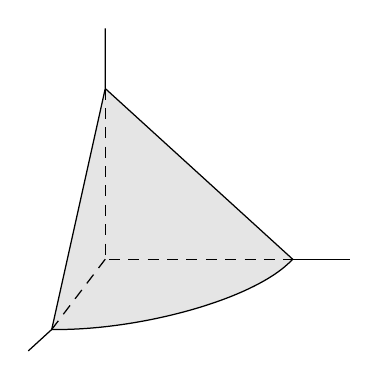
\begin{tikzpicture}[line width=.45pt,scale=.85]
  \fill[gray!20] (0,2.8) -- (-.8,-.8)
    .. controls (.5,-.82) and (2.25,-.35) .. (2.8,.25) -- cycle;
  \draw (0,3.7) -- (0,2.8) -- (-.8,-.8)
    .. controls (.5,-.82) and (2.25,-.35) .. (2.8,.25) -- (0,2.8);
  \draw (-1.15,-1.12) -- (-.8,-.8);
  \draw (2.8,.25) -- (3.65,.25);
  \draw[dash pattern=on 4pt off 3pt] (0,2.8) -- (0,.25) -- (2.8,.25);
  \draw[dash pattern=on 4pt off 3pt] (0,.25) -- (-.8,-.8);
\end{tikzpicture}
\end{center}
\nopagebreak[4]
(A) 14 斛　(B) 22 斛　(C) 36 斛　(D) 66 斛

\Needspace{4\baselineskip}
\textbf{解析}

四分之一圆周长 $\pi r/2=8$，取题给 $\pi\approx3$，得 $r\approx16/3$。米堆体积 $\frac14\cdot\frac13\pi r^2\cdot5\approx35.56$ 立方尺，除以 1.62 约为 21.95 斛。

\gkanswer{答案：B，约 $22$ 斛}

\end{answer}
\begin{answer}
\gksolhead{7}{}

\textbf{题目}：

已知 $\{a_n\}$ 是公差为 1 的等差数列，$S_n$ 为 $\{a_n\}$ 的前 $n$ 项和，若 $S_8=4S_4$，则 $a_{10}=$（　）

(A) $\frac{17}2$　(B) $\frac{19}2$　(C) 10　(D) 12

\Needspace{4\baselineskip}
\textbf{解析}

设首项 $a_1$，$S_8=8a_1+28$、$4S_4=16a_1+24$，故 $a_1=\frac12$，$a_{10}=\frac{19}2$。

\gkanswer{答案：B，$\frac{19}2$}

\end{answer}
\begin{answer}
\gksolhead{8}{}

\textbf{题目}：

函数 $f(x)=\cos(\omega x+\varphi)$ 的部分图象如图所示，则 $f(x)$ 的单调递减区间为（　）
\nopagebreak[4]
\begin{center}% [fig-q08-cosine], fixed PDF p.1 / printed 963.
% Smooth visible contour reconstructed with layout-only Bezier controls.
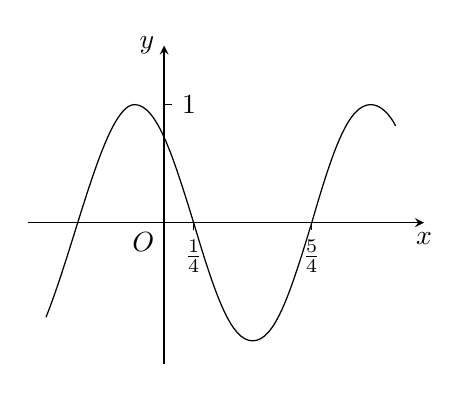
\begin{tikzpicture}[>=stealth,line width=.45pt,x=1.5cm,y=1.5cm]
  \draw[->] (-1.15,0) -- (2.2,0) node[below] {$x$};
  \draw[->] (0,-1.2) -- (0,1.5) node[left] {$y$};
  \node[below left] at (0,0) {$O$};
  \draw (0,1) -- (.07,1) node[right] {$1$};
  \draw (.25,0) -- (.25,-.06) node[below] {$\frac14$};
  \draw (1.25,0) -- (1.25,-.06) node[below] {$\frac54$};
  \draw (-1,-.8) .. controls (-.74,-.15) and (-.50,1) .. (-.25,1)
    .. controls (-.06,1) and (.08,.55) .. (.25,0)
    .. controls (.44,-.64) and (.57,-1) .. (.75,-1)
    .. controls (.94,-1) and (1.07,-.59) .. (1.25,0)
    .. controls (1.43,.62) and (1.56,1) .. (1.75,1)
    .. controls (1.83,1) and (1.91,.92) .. (1.96,.82);
\end{tikzpicture}
\end{center}
\nopagebreak[4]
(A) $(k\pi-\frac14,k\pi+\frac34),k\in\mathbf Z$　(B) $(2k\pi-\frac14,2k\pi+\frac34),k\in\mathbf Z$

(C) $(k-\frac14,k+\frac34),k\in\mathbf Z$　(D) $(2k-\frac14,2k+\frac34),k\in\mathbf Z$

\Needspace{4\baselineskip}
\textbf{解析}

图中 $x=\frac14$ 处向下过零，$x=\frac54$ 处向上过零，间距为半周期 1；相邻最大值至最小值区间为 $(-\frac14,\frac34)$，周期 2。

\gkanswer{答案：D}

\end{answer}
\begin{answer}
\gksolhead{9}{}

\textbf{题目}：

执行如图的程序框图，如果输入的 $t=0.01$，则输出的 $n=$（　）
\nopagebreak[4]
\begin{center}% Source-faithful content draft for [fig-q09-flowchart], PDF p.1 / printed p.963.
% Uses only basic TikZ paths and nodes; scaling/spacing are presentational.
\begin{tikzpicture}[>=stealth, every node/.style={font=\small}]
  \draw[rounded corners=5pt] (-0.52,0.05) rectangle (0.52,0.55);
  \node at (0,0.30) {开始};
  \draw[->] (0,0.05) -- (0,-0.45);
  \draw (-0.62,-0.45) -- (0.82,-0.45) -- (0.62,-0.95) -- (-0.82,-0.95) -- cycle;
  \node at (0,-0.70) {输入 $t$};
  \draw[->] (0,-0.95) -- (0,-1.45);
  \draw (-1.70,-1.45) rectangle (1.70,-2.00);
  \node at (0,-1.725) {$S=1,\ n=0,\ m=\frac12$};
  \draw[->] (0,-2.00) -- (0,-2.50);
  \draw (-0.92,-2.50) rectangle (0.92,-3.00);
  \node at (0,-2.75) {$S=S-m$};
  \draw[->] (0,-3.00) -- (0,-3.48);
  \draw (-1.50,-3.48) rectangle (1.50,-4.03);
  \node at (0,-3.755) {$m=\frac m2,\ n=n+1$};
  \draw[->] (0,-4.03) -- (0,-4.53);
  \draw (-1.08,-4.85) -- (0,-4.53) -- (1.08,-4.85) -- (0,-5.17) -- cycle;
  \node at (0,-4.85) {$S>t$};
  \draw[->] (-1.08,-4.85) -- (-2.05,-4.85) -- (-2.05,-2.25) -- (0,-2.25) -- (0,-2.50);
  \node[left] at (-1.08,-4.72) {是};
  \draw[->] (0,-5.17) -- (0,-5.65);
  \node[right] at (0.06,-5.40) {否};
  \draw (-0.62,-5.65) -- (0.82,-5.65) -- (0.62,-6.15) -- (-0.82,-6.15) -- cycle;
  \node at (0,-5.90) {输出 $n$};
  \draw[->] (0,-6.15) -- (0,-6.62);
  \draw[rounded corners=5pt] (-0.52,-7.12) rectangle (0.52,-6.62);
  \node at (0,-6.87) {结束};
\end{tikzpicture}
\end{center}
\nopagebreak[4]
(A) 5　(B) 6　(C) 7　(D) 8

\Needspace{4\baselineskip}
\textbf{解析}

每轮先从 $S$ 减去 $m$，再令 $m$ 减半、$n$ 加一；第 $n$ 轮后 $S=2^{-n}$。$2^{-6}=0.015625>0.01$，$2^{-7}=0.0078125\leq0.01$，输出 $n=7$。

\gkanswer{答案：C，$7$}

\end{answer}
\begin{answer}
\gksolhead{10}{}

\textbf{题目}：

已知函数 $f(x)=\begin{cases}2^{x-1}-2,&x\leqslant1,\\-\log_2(x+1),&x>1,\end{cases}$ 且 $f(a)=-3$，则 $f(6-a)=$（　）

(A) $-\frac74$　(B) $-\frac54$　(C) $-\frac34$　(D) $-\frac14$

\Needspace{4\baselineskip}
\textbf{解析}

$x\leq1$ 时 $2^{x-1}-2>-2$，所以 $f(a)=-3$ 只能来自 $a>1$。$-\log_2(a+1)=-3$ 得 $a=7$，$f(6-a)=f(-1)=2^{-2}-2=-\frac74$。

\gkanswer{答案：A，$-\frac74$}

\end{answer}
\begin{answer}
\gksolhead{11}{}

\textbf{题目}：

圆柱被一个平面截去一部分后与半球（半径为 $r$）组成一个几何体，该几何体三视图中的正视图和俯视图如图所示。若该几何体的表面积为 $16+20\pi$，则 $r=$（　）
\nopagebreak[4]
\begin{center}% [fig-q11-front], fixed PDF p.1 / printed 963.
\begin{tikzpicture}[>=stealth,line width=.45pt]
  \draw (0,0) circle (1);
  \draw (-1,0) -- (1,0);
  \draw[thin] (-1,0) -- (-1,1.45) (1,0) -- (1,1.45);
  \draw[<->] (-1,1.25) -- (1,1.25) node[midway,above] {$2r$};
  \draw[thin] (1,0) -- (1.4,0) (0,-1) -- (1.4,-1);
  \draw[<->] (1.23,0) -- (1.23,-1) node[midway,right] {$r$};
  \node[below] at (0,-1.12) {正视图};
\end{tikzpicture}
\end{center}
\nopagebreak[4]
\nopagebreak[4]
\begin{center}% [fig-q11-top], fixed PDF p.1 / printed 963.
\begin{tikzpicture}[>=stealth,line width=.45pt]
  \draw (-1,0) arc[start angle=180,end angle=0,radius=1];
  \draw (-1,0) -- (1,0) -- (1,-2) -- (-1,-2) -- cycle;
  \draw[thin] (0,1) -- (-1.3,1) (-1,0) -- (-1.3,0);
  \draw[<->] (-1.2,0) -- (-1.2,1) node[midway,left] {$r$};
  \draw[thin] (1,0) -- (1.4,0) (1,-2) -- (1.4,-2);
  \draw[<->] (1.23,0) -- (1.23,-2) node[midway,right] {$2r$};
  \node[below] at (0,-2.12) {俯视图};
\end{tikzpicture}
\end{center}
\nopagebreak[4]
(A) 1　(B) 2　(C) 4　(D) 8

\Needspace{4\baselineskip}
\textbf{解析}

按两个投影视图，外露曲面由半圆柱侧面 $2\pi r^2$ 与半球面 $2\pi r^2$ 构成，外露圆形端/底面合计 $\pi r^2$，平面截面为 $4r^2$；表面积 $5\pi r^2+4r^2=16+20\pi$，所以 $r=2$。

\gkanswer{答案：B，$2$}

\end{answer}
\begin{answer}
\gksolhead{12}{}

\textbf{题目}：

设函数 $y=f(x)$ 的图象与 $y=2^{x+a}$ 的图象关于直线 $y=-x$ 对称，且 $f(-2)+f(-4)=1$，则 $a=$（　）

(A) $-1$　(B) 1　(C) 2　(D) 4

\Needspace{4\baselineskip}
\textbf{解析}

对称变换 $(u,v)\mapsto(-v,-u)$ 把 $v=2^{u+a}$ 变成 $f(x)=a-\log_2(-x)$（$x<0$）。于是 $(a-1)+(a-2)=1$，得 $a=2$。

\gkanswer{答案：C，$2$}

\end{answer}
\begin{answer}
\gksolhead{13}{}

\textbf{题目}：

数列 $\{a_n\}$ 中 $a_1=2$，$a_{n+1}=2a_n$，$S_n$ 为 $\{a_n\}$ 的前 $n$ 项和，若 $S_n=126$，则 $n=$\gkblank{}。

\Needspace{4\baselineskip}
\textbf{解析}

$a_n=2^n$，$S_n=2^{n+1}-2=126$，故 $n=6$。

\gkanswer{答案：$6$}

\end{answer}
\begin{answer}
\gksolhead{14}{}

\textbf{题目}：

已知函数 $f(x)=ax^3+x+1$ 的图象在点 $(1,f(1))$ 处的切线过点 $(2,7)$，则 $a=$\gkblank{}。

\Needspace{4\baselineskip}
\textbf{解析}

$f(1)=a+2$、$f'(1)=3a+1$。切线过 $(2,7)$ 给出 $7=(a+2)+(3a+1)$，故 $a=1$。

\gkanswer{答案：$1$}

\end{answer}
\begin{answer}
\gksolhead{15}{}

\textbf{题目}：

若 $x,y$ 满足约束条件 $\begin{cases}x+y-2\leqslant0,\\x-2y+1\leqslant0,\\2x-y+2\geqslant0,\end{cases}$ 则 $z=3x+y$ 的最大值为\gkblank{}。

\Needspace{4\baselineskip}
\textbf{解析}

三条边界两两相交并满足全部约束的顶点为 $(-1,0),(0,2),(1,1)$；$3x+y$ 分别为 $-3,2,4$，最大为 4。

\gkanswer{答案：$4$}

\end{answer}
\begin{answer}
\gksolhead{16}{}

\textbf{题目}：

已知 $F$ 是双曲线 $C:x^2-\frac{y^2}{8}=1$ 的右焦点，$P$ 是 $C$ 左支上一点，$A(0,6\sqrt6)$，当 $\triangle APF$ 周长最小时，该三角形的面积为\gkblank{}。

\Needspace{4\baselineskip}
\textbf{解析}

左焦点 $F'=(-3,0)$、右焦点 $F=(3,0)$，左支上 $PF-PF'=2$。周长 $AP+PF+AF=AP+PF'+2+AF$，由三角不等式在 $P$ 落于线段 $AF'$ 与左支的交点时最小。$AF'$ 的直线为 $y=2\sqrt6(x+3)$，与双曲线左支相交于 $P=(-2,2\sqrt6)$。由坐标行列式，$[APF]=\frac12|\det(P-A,F-A)|=12\sqrt6$。

\gkanswer{答案：$12\sqrt6$}

\end{answer}
\begin{answer}
\gksolhead{17}{}

\textbf{题目}：

已知 $a,b,c$ 分别是 $\triangle ABC$ 内角 $A,B,C$ 的对边，$\sin^2B=2\sin A\sin C$。

(1) 若 $a=b$，求 $\cos B$；

(2) 若 $B=90^\circ$，且 $a=\sqrt2$，求 $\triangle ABC$ 的面积。

\Needspace{4\baselineskip}
\textbf{解析}

正弦定理将 $\sin^2B=2\sin A\sin C$ 化为 $b^2=2ac$。

\gksubpart{(1)}

$a=b$，所以 $b=2c$，余弦定理给 $\cos B=(a^2+c^2-b^2)/(2ac)=\frac14$。

\gksubpart{(2)}

$B=90^\circ$ 又给 $b^2=a^2+c^2$，与 $b^2=2ac$ 合并得 $(a-c)^2=0$。$a=c=\sqrt2$，面积 $ac/2=1$。

\gkanswer{答案（1）：$\frac14$}

\gkanswer{答案（2）：$1$}

\end{answer}
\begin{answer}
\gksolhead{18}{}

\textbf{题目}：

如图，四边形 $ABCD$ 为菱形，$G$ 为 $AC$ 与 $BD$ 的交点，$BE\perp$ 平面 $ABCD$。

(1) 证明：平面 $AEC\perp$ 平面 $BED$；

(2) 若 $\angle ABC=120^\circ$，$AE\perp EC$，三棱锥 $E-ACD$ 的体积为 $\frac{\sqrt6}{3}$，求该三棱锥的侧面积。
\nopagebreak[4]
\begin{center}% [fig-q18-rhombus], fixed PDF p.1 / printed 963.
% These are page-layout projections, not spatial coordinates or derived edges.
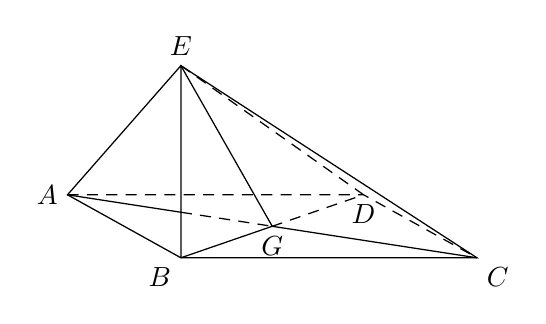
\begin{tikzpicture}[line width=.45pt,scale=.8]
  \coordinate (A) at (0,1);
  \coordinate (B) at (1.8,0);
  \coordinate (C) at (6.5,0);
  \coordinate (D) at (4.7,1);
  \coordinate (G) at (3.25,.5);
  \coordinate (E) at (1.8,3.05);
  \draw (E) -- (A) -- (B) -- (C) -- (E) -- (B);
  \draw (E) -- (G) -- (C) (B) -- (G);
  % Source AC is solid from A to EB, hidden from EB to G, solid G to C.
  \draw (A) -- (1.8,.72308);
  \draw[dash pattern=on 4pt off 3pt] (1.8,.72308) -- (G);
  \draw[dash pattern=on 4pt off 3pt] (A) -- (D) -- (C) (E) -- (D) -- (G);
  \node[left] at (A) {$A$};
  \node[below left] at (B) {$B$};
  \node[below right] at (C) {$C$};
  \node[below] at (D) {$D$};
  \node[above] at (E) {$E$};
  \node[below] at (G) {$G$};
\end{tikzpicture}
\end{center}
\nopagebreak[4]
\Needspace{4\baselineskip}
\textbf{解析}

\gksubpart{(1)}

菱形对角线 $AC\perp BD$；因 $BE\perp$ 底面，也有 $AC\perp BE$。$BD,BE$ 是平面 $BED$ 内相交的两条直线，故 $AC\perp$ 平面 $BED$。由于 $AC\subset$ 平面 $AEC$，两平面垂直。

\gksubpart{(2)}

设 $G=(0,0,0)$，$A=(-p,0,0)$、$C=(p,0,0)$、$B=(0,-q,0)$、$D=(0,q,0)$、$E=(0,-q,h)$，其中 $p,q,h>0$。$\angle ABC=120^\circ$ 给 $p^2=3q^2$；$AE\perp EC$ 给 $h^2=p^2-q^2=2q^2$。$[ACD]=pq$，所以 $V_{E-ACD}=pqh/3=\sqrt6q^3/3=\sqrt6/3$，即 $q=1$、$p=\sqrt3$、$h=\sqrt2$。侧面 $EAC$ 面积 $p\sqrt{q^2+h^2}=3$；另两侧面 $EAD,ECD$ 各为 $\sqrt5$，合计 $3+2\sqrt5$。

\gkanswer{答案（1）：两平面垂直，见证明}

\gkanswer{答案（2）：$3+2\sqrt5$}

\end{answer}
\begin{answer}
\gksolhead{19}{}

\textbf{题目}：

某公司为确定下一年度投入某产品的宣传费，需了解年宣传费 $x$（单位：千元）对年销售量 $y$（单位：t）和年利润 $z$（单位：千元）的影响。对近 8 年的年宣传费 $x_i$ 和年销售量 $y_i$（$i=1,2,\cdots,8$）数据作了初步处理，得到下面的散点图及一些统计量的值。
\nopagebreak[4]
\begin{center}% [fig-q19-scatter], fixed PDF p.2 / printed 964.
% Eight unlabelled squares are approximate visual placements, not raw data.
\begin{tikzpicture}[>=stealth,line width=.4pt,x=.23cm,y=.023cm,
  every node/.style={font=\small}]
  \draw[->] (34,480) -- (62,480);
  \draw[->] (34,480) -- (34,640);
  \foreach \x in {34,36,...,56} {
    \draw (\x,480) -- (\x,484);
    \node[below] at (\x,480) {\x};
  }
  \foreach \y in {480,500,...,620} {
    \draw (34,\y) -- (34.4,\y);
    \node[left] at (34,\y) {\y};
  }
  \node[above right] at (34,635) {年销售量/t};
  \node[above] at (62,480) {年宣传费/千元};
  \foreach \x/\y in {38/502,40/534,44/564,46/576,48/590,50/596,52/600,56/604} {
    \fill (\x,\y) ++(-1pt,-1pt) rectangle ++(2pt,2pt);
  }
\end{tikzpicture}
\end{center}
\nopagebreak[4]
\begin{center}
\begin{tabular}{rrrrr}
\toprule
$\bar x$ & $\bar y$ & $\bar w$ & $\sum_{i=1}^{8}(x_i-\bar x)^2$ & $\sum_{i=1}^{8}(w_i-\bar w)^2$ \\
\midrule
46.6 & 563 & 6.8 & 289.8 & 1.6 \\
\bottomrule
\end{tabular}
\end{center}

\begin{center}
\begin{tabular}{rr}
\toprule
$\sum_{i=1}^{8}(x_i-\bar x)(y_i-\bar y)$ & $\sum_{i=1}^{8}(w_i-\bar w)(y_i-\bar y)$ \\
\midrule
1.469 & 108.8 \\
\bottomrule
\end{tabular}
\end{center}

表中 $w_i=\sqrt{x_i}$，$\bar w=\frac18\sum_{i=1}^{8}w_i$。

(1) 根据散点图判断，$y=a+bx$ 与 $y=c+d\sqrt x$ 哪一个适宜作为年销售量 $y$ 关于年宣传费 $x$ 的回归方程类型？（给出判断即可，不必说明理由）

(2) 根据 (1) 的判断结果及表中数据，建立 $y$ 关于 $x$ 的回归方程；

(3) 已知这种产品的年利润 $z$ 与 $x,y$ 的关系为 $z=0.2y-x$。根据 (2) 的结果回答下列问题：

① 年宣传费 $x=49$ 时，年销售量及年利润的预报值是多少？

② 年宣传费 $x$ 为何值时，年利润的预报值最大？

附：对于一组数据 $(u_1,v_1),(u_2,v_2),\cdots,(u_n,v_n)$，其回归直线 $v=\alpha+\beta u$ 的斜率和截距的最小二乘估计分别为 $\hat\beta=\frac{\sum_{i=1}^{n}(u_i-\bar u)(v_i-\bar v)}{\sum_{i=1}^{n}(u_i-\bar u)^2}$，$\hat\alpha=\bar v-\hat\beta\bar u$。

\Needspace{4\baselineskip}
\textbf{解析}

\gksubpart{(1)}

散点随 $x$ 增加而上升，增速逐渐减缓，选择平方根模型 $y=c+d\sqrt x$。

\gksubpart{(2)}

令 $w=\sqrt x$，用对应列建立线性回归：$\widehat d=108.8/1.6=68$，$\widehat c=563-68\cdot6.8=100.6$，从而 $\widehat y=100.6+68\sqrt x$。源表另一列印作 \texttt{1.469}，量级疑点保留，未参与这个模型。

\gksubpart{(3)}

① $x=49$ 时 $\widehat y=576.6$ t，$\widehat z=0.2\cdot576.6-49=66.32$ 千元。

② $\widehat z=20.12+13.6\sqrt x-x=66.36-(\sqrt x-6.8)^2$，在 $x=46.24$ 千元时最大。

\gkanswer{答案（1）：$y=c+d\sqrt x$}

\gkanswer{答案（2）：$\widehat y=100.6+68\sqrt x$}

\gkanswer{答案（3）：① $576.6$ t、$66.32$ 千元；② $x=46.24$ 千元}

\end{answer}
\begin{answer}
\gksolhead{20}{}

\textbf{题目}：

已知过点 $A(0,1)$ 且斜率为 $k$ 的直线 $l$ 与圆 $C:(x-2)^2+(y-3)^2=1$ 交于 $M,N$ 两点。

(1) 求 $k$ 的取值范围；

(2) 若 $\overrightarrow{OM}\cdot\overrightarrow{ON}=12$，其中 $O$ 为坐标原点，求 $|MN|$。

\Needspace{4\baselineskip}
\textbf{解析}

\gksubpart{(1)}

圆心 $(2,3)$ 到直线 $y=kx+1$ 的距离为 $|2k-2|/\sqrt{1+k^2}$。要有两个交点，须此距离小于半径 $1$，即 $3k^2-8k+3<0$，故两根之间为所求范围。

\gksubpart{(2)}

代入圆方程得 $(1+k^2)x^2-4(1+k)x+7=0$。设交点横坐标为 $x_1,x_2$，则 $x_1+x_2=4(1+k)/(1+k^2)$，$x_1x_2=7/(1+k^2)$。点积为 $(1+k^2)x_1x_2+k(x_1+x_2)+1=8+4k(1+k)/(1+k^2)$。令其等于 $12$ 得 $k=1$；此时直线过圆心，$MN$ 为直径，长 $2$。

\gkanswer{答案（1）：$\frac{4-\sqrt7}{3}<k<\frac{4+\sqrt7}{3}$}

\gkanswer{答案（2）：$2$}

\end{answer}
\begin{answer}
\gksolhead{21}{}

\textbf{题目}：

设函数 $f(x)=e^{2x}-a\ln x$。

(1) 讨论 $f(x)$ 的导函数 $f'(x)$ 的零点的个数；

(2) 证明：当 $a>0$ 时，$f(x)\geqslant2a+a\ln\frac2a$。

\Needspace{4\baselineskip}
\textbf{解析}

\gksubpart{(1)}

定义域为 $x>0$，$f'(x)=(2xe^{2x}-a)/x$。函数 $2xe^{2x}$ 在正半轴严格递增且值域为 $(0,+\infty)$，所以 $a\le0$ 时导函数无零点，$a>0$ 时有且仅有一个。

\gksubpart{(2)}

\Needspace{5\baselineskip}
令 $t=2x>0$。指数函数切线不等式给出 $e^t\ge a(t+1-\ln a)$，且 $t-\ln t\ge1$。于是
\nopagebreak[4]
\[f(x)=e^t-a\ln(t/2)\ge a(t-\ln t+1+\ln2-\ln a)\ge2a+a\ln(2/a).\]
两次等号同时成立须 $t=\ln a=1$，即 $a=e,x=1/2$。

\gkanswer{答案（1）：$a\le0$ 时无零点，$a>0$ 时恰有一个零点}

\gkanswer{答案（2）：不等式成立，见证明}

\end{answer}
\begin{answer}
\gksolhead{22}{}

\textbf{题目}：

如图，$AB$ 是 $\odot O$ 的直径，$AC$ 是 $\odot O$ 的切线，$BC$ 交 $\odot O$ 于点 $E$。

(1) 若 $D$ 为 $AC$ 的中点，证明：$DE$ 是 $\odot O$ 的切线；

(2) 若 $OA=\sqrt3 CE$，求 $\angle ACB$ 的大小。
\nopagebreak[4]
\begin{center}% [fig-q22-circle], fixed PDF p.2 / printed 964.
% Layout-only circle/secant construction; DE is visible in the source.
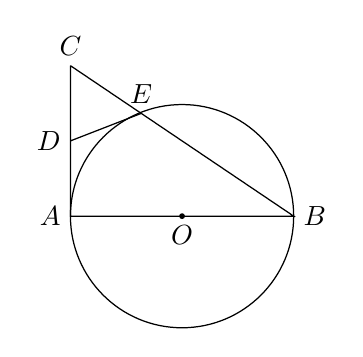
\begin{tikzpicture}[line width=.45pt,scale=1.05]
  \coordinate (A) at (-1.35,0);
  \coordinate (B) at (1.35,0);
  \coordinate (C) at (-1.35,1.82);
  \coordinate (D) at (-1.35,.91);
  \coordinate (E) at (-.4935,1.2426);
  \draw (0,0) circle (1.35);
  \draw (C) -- (A) -- (B) -- (C) (D) -- (E);
  \fill (0,0) circle (1pt);
  \node[left] at (A) {$A$};
  \node[right] at (B) {$B$};
  \node[above] at (C) {$C$};
  \node[left] at (D) {$D$};
  \node[above] at (E) {$E$};
  \node[below] at (0,0) {$O$};
\end{tikzpicture}
\end{center}
\nopagebreak[4]
\Needspace{4\baselineskip}
\textbf{解析}

\gksubpart{(1)}

$AB$ 为直径且 $E$ 在圆上，$AE\perp BE$；$C,E,B$ 共线，所以 $AE\perp CE$。在直角三角形 $AEC$ 中，$D$ 为斜边 $AC$ 的中点，于是 $DA=DE$。又 $OA=OE$、$OD$ 公共，三角形 $OAD$ 与 $OED$ 由三边对应相等而全等。$OA\perp AD$（$AC$ 在 $A$ 相切），故 $OE\perp ED$，$DE$ 为切线。

\gksubpart{(2)}

记 $R=OA$、$L=CB$，由切割线定理 $CA^2=CE\cdot CB=RL/\sqrt3$。直角三角形 $ACB$ 中 $CA^2=L^2-(2R)^2$，故 $(L/R)^2-(L/R)/\sqrt3-4=0$。正根 $L/R=4/\sqrt3$，从而 $\sin\angle ACB=AB/CB=2R/L=\sqrt3/2$。该角为锐角，故为 $60^\circ$。

\gkanswer{答案（1）：$DE$ 为切线，见证明}

\gkanswer{答案（2）：$60^\circ$}

\end{answer}
\begin{answer}
\gksolhead{23}{}

\textbf{题目}：

在直角坐标系 $xOy$ 中，直线 $C_1:x=-2$，圆 $C_2:(x-1)^2+(y-2)^2=1$，以坐标原点为极点，$x$ 轴的正半轴为极轴建立极坐标系。

(1) 求 $C_1,C_2$ 的极坐标方程；

(2) 若直线 $C_3$ 的极坐标方程为 $\theta=\frac\pi4$（$\rho\in\mathbf R$），设 $C_2$ 与 $C_3$ 的交点为 $M,N$，求 $\triangle C_2MN$ 的面积。

\Needspace{4\baselineskip}
\textbf{解析}

\gksubpart{(1)}

代入 $x=\rho\cos\theta,y=\rho\sin\theta$，得 $C_1:\rho\cos\theta=-2$，$C_2:\rho^2-2\rho\cos\theta-4\rho\sin\theta+4=0$。

\gksubpart{(2)}

原文定义“圆 $C_2$”而未定义同名顶点，却要求 $\triangle C_2MN$ 的面积，故该项为 U，不能无条件把圆替换为圆心。若条件性解释为圆心 $(1,2)$，直线 $C_3$ 为 $y=x$，交点 $(1,1),(2,2)$，弦长 $\sqrt2$、圆心到弦距离 $1/\sqrt2$，于是条件性面积为 $1/2$。题面照原文保留。

\gkanswer{答案（1）：$C_1:\rho\cos\theta=-2$；$C_2:\rho^2-2\rho\cos\theta-4\rho\sin\theta+4=0$}

\gkanswer{答案（2）：U：原文未定义三角形顶点 $C_2$；若指圆心则面积为 $\frac12$（条件性结论）}

\end{answer}
\begin{answer}
\gksolhead{24}{}

\textbf{题目}：

已知函数 $f(x)=|x+1|-2|x-a|$，$a>0$。

(1) 当 $a=1$ 时，求不等式 $f(x)>1$ 的解集；

(2) 若 $f(x)$ 的图象与 $x$ 轴围成的三角形面积大于 6，求 $a$ 的取值范围。

\Needspace{4\baselineskip}
\textbf{解析}

\gksubpart{(1)}

当 $a=1$，在 $x<-1$、$-1\leq x\leq1$、$x>1$ 三段分别有 $f=x-3,3x-1,3-x$；解 $f>1$ 得 $(2/3,2)$。

\gksubpart{(2)}

一般 $a>0$ 时，两零点分别为 $x_L=(2a-1)/3$ 与 $x_R=1+2a$，顶点 $(a,a+1)$。所围三角形面积 $\frac12(x_R-x_L)(a+1)=\frac23(a+1)^2$，大于 6 当且仅当 $a>2$。

\gkanswer{答案（1）：$(\frac23,2)$}

\gkanswer{答案（2）：$a>2$}

\end{answer}